\documentclass[11pt]{article}
\usepackage[margin=1in]{geometry}
\usepackage{amsmath,amssymb}
\usepackage{graphicx}
\usepackage{booktabs}
\usepackage{array}
\usepackage{caption}
\usepackage[hidelinks]{hyperref}
\usepackage{xcolor}
\usepackage{titlesec}
\usepackage{enumitem}
\usepackage{microtype}

\titleformat{\section}{\normalfont\large\bfseries}{\thesection}{1em}{}
\titleformat{\subsection}{\normalfont\normalsize\bfseries}{\thesubsection}{1em}{}
\setlength{\parskip}{0.4em}
\setlength{\parindent}{0pt}
\captionsetup{font=small,labelfont=bf}
\newcommand{\rid}[1]{\texttt{\small #1}}

\title{\bfseries The Left-Hemisphere Complement of the \textit{Drosophila}\\
Figure-Ground Course-Control Circuit}
\author{Stage 8, Connectomics platform \\ \small FlyWire FAFB v783 and male whole-CNS (male-cns:v1.0)}
\date{}

\begin{document}
\maketitle

\begin{abstract}
\noindent
The companion analysis of the adult \textit{Drosophila} brain established, in the right optic
lobe of the FlyWire FAFB connectome, a two-stage figure-ground course-control circuit in which a
left-soma centrifugal horizontal cell (VCH) presynaptically gates the front-to-back T4a terminals
that drive a one-hundred-cell cholinergic LLPC1 sheet, whose dominant excitatory readout Nod1
relays a figure-motion signal to the wing-steering command neuron DNp26. That study analysed a
single hemisphere and a single horizontal direction, and explicitly did not determine whether the
left optic lobe contains the homologous circuit. Here we resolve that question. Working from the
same connectome and the same synapse-resolution methods, and using the right-hemisphere
derivation as a reproduced positive control, we determine the precise left-side cell identities,
demonstrate that they reproduce every internal feature of the right circuit, and show that the
two hemispheres form a complementary pair: the left circuit is gated by the right-soma VCH,
reads the same front-to-back T4a channel under the same back-to-front opponent inhibition,
pools its inputs retinotopically, routes its output through Nod1 to DNp26, and ultimately steers
the wing on the body side opposite to the one steered by the right circuit. The left LLPC1 sheet
comprises eighty-six cells reached by four hundred and eleven VCH-gated left T4a neurons. We
also re-examine, and qualify, the previously assumed correspondence between Nod1 and the
Egelhaaf (1985) figure-detection cell FD1: Nod1 satisfies every measurable functional property of
FD1 and is the best functional match among the candidate cells, but it is a central-brain
projection neuron rather than a lobula-plate tangential cell, so it is the functional and
anatomical correlate of FD1 rather than that cell type itself. Two quantitative differences
between the hemispheres are reported in full. The result identifies the left-hemisphere figure
circuit cell by cell and demonstrates that the figure-ground course-control system is bilaterally
organised as a mirror-symmetric pair of single-wing steering channels.
\end{abstract}

\section{Introduction}

Relative motion breaks camouflage. A textured object that is invisible against a matched
background becomes detectable when it moves with a velocity or phase different from the
surrounding panorama, and flies use this cue to track figures and to fixate them with corrective
turns. The companion connectomic study traced the pathway that converts a population of local
motion detectors into a spatially localised figure signal and delivers that signal to descending
motor control. In the right optic lobe of the adult female FlyWire FAFB connectome, the pathway
begins with the centrifugal horizontal cell VCH, which pools wide-field T4/T5 motion and feeds
GABAergic inhibition back onto the front-to-back (lobula-plate layer-a) T4a axon terminals that
drive a one-hundred-cell cholinergic LLPC1 sheet. The sheet reads this gated, locally pooled
signal retinotopically, integrates non-direction-selective form input from the lobula, and is
regulated by opponent-direction LPi15 inhibition and recurrent PVLP011 feedback. The dominant
excitatory readout of the sheet is the central-brain projection neuron Nod1, which relays the
figure signal almost entirely to steering descending neurons and principally to DNp26, the
wing-steering command neuron, whose action in the male whole-CNS connectome biases the
contralateral wing through the hg1 and i1 steering muscles.

That study was, by its own statement, the front-to-back right-side exemplar of a bilateral,
multi-direction system, and it did not establish whether the left optic lobe contains the
homologous circuit. The optic lobes are mirror-symmetric, so the existence of a left-hemisphere
counterpart is plausible, but plausibility is not demonstration. The present work treats the
existence of a left-hemisphere figure circuit as the question to be answered rather than as a
premise. We ask three things in order. First, does the left optic lobe contain a circuit with the
same architecture as the right circuit, and if so, which exact neurons constitute it. Second, are
the internal properties of that left circuit quantitatively the same as those of the right
circuit. Third, is the left circuit the complement of the right circuit in the specific sense
that matters for behaviour, namely that the two circuits steer opposite wings so that a figure on
one side of the visual field and a figure on the other drive opposite corrective turns.

A second matter required attention before the comparison could be interpreted. The companion
study identified the cholinergic readout Nod1 with the figure-detection cell FD1 described by
Egelhaaf (1985), and the project's downstream analyses adopted Nod1 as the FD1 reference without
an independent test of that identity. Neither the companion paper nor Egelhaaf states the
identity explicitly, and there is an anatomical tension, because Egelhaaf's FD1 is a large-field
lobula-plate tangential cell whereas Nod1 in the connectome is annotated as a central-brain
projection neuron downstream of the LLPC1 sheet. We therefore re-examined the Nod1 to FD1
correspondence on the right hemisphere before constructing any left-hemisphere counterpart, so
that the figure-detection labels carried into the left analysis would be defined and qualified
rather than assumed.

\section{Methods}

All optic-lobe, sheet, and descending-neuron measurements were computed from the adult female
FlyWire FAFB connectome at materialization version 783, using chemical synapses from the
\texttt{synapses\_nt\_v1} table with no cleft-score threshold, and the hierarchical cell-type,
super-class, side, and neurotransmitter annotations of the whole-brain annotation framework. The
motor read-out used the male whole-CNS connectome (male-cns:v1.0), which contains both the brain
and the ventral nerve cord and therefore links descending-neuron cell types to their
motor-neuron targets. Synapse counts are used as anatomical evidence and not as direct measures
of synaptic efficacy. Predicted neurotransmitter is used as an anatomical annotation and not as
an established transmitter identity. These choices reproduce the companion study's published
synapse totals exactly, which is the basis on which the right-hemisphere derivation serves as a
positive control here.

The central methodological decision was to compute both hemispheres through one parametrised
analysis path. Centrifugal horizontal cells cross the midline: a VCH or DCH cell whose soma lies
on one side has its arbor in the opposite optic lobe and gates that lobe's sheet. The right
sheet is therefore gated by the left-soma VCH (the cell the companion study analysed,
\rid{720575940627706398}), and the left sheet is gated by the right-soma VCH
(\rid{720575940627502338}). We encoded each hemisphere as a side configuration consisting of the
sheet side, the gating-soma side, the gating VCH and DCH root identifiers, the front-to-back
exemplar subtype T4a, and the opponent layer-b subtype. The same code, given the right
configuration, reproduces the companion study to the digit; given the left configuration, it
derives the homologous left quantities. Because every left and right number passes through
identical code, any difference between them is a property of the connectome and not of the
analysis. The two-hemisphere comparison was further protected by an explicit cache key on the
sheet side, so that a left derivation following a right derivation could not silently reuse the
right sheet.

The left sheet was defined exactly as the right sheet is defined. We took the front-to-back T4a
neurons on the left side that are postsynaptic to the right-soma VCH (the VCH-gated left T4a),
followed their output to left-side LLPC1 cells, and called the set of LLPC1 cells reached in this
way the left sheet. This is the homologous construction to the companion study's right sheet of
one hundred LLPC1 cells reached by four hundred and fifty-four VCH-gated right T4a neurons.

Statistical procedures followed the companion study. Pooling locality was tested against an
in-degree-preserving permutation null over five hundred permutations, with significance reported
as a z-score against the null distribution and a permutation p-value. Synapse-location analyses
snapped each synapse to its three-dimensional position in micrometres and computed Euclidean
distances; paired synapse-location comparisons used the two-sided Wilcoxon signed-rank test
across neurons. Wing laterality in the male whole-CNS connectome was read from the motor neuron
soma side, which records the wing a motor neuron innervates, and was tested against a permutation
null over the motor-neuron soma-side labels.

The investigation was structured so that a negative or partial result could be reached and
reported. Before the full derivation, a low-cost screen walked the seven stages of the right
circuit on the left side and labelled each present, weak, or absent, with absolute floors so that
a near-zero left value or a qualitatively different wiring would register as absent rather than
being absorbed into a tolerance. The full derivation then ran the nine internal stages on both
sides, computed the explicit left-to-right comparisons and the wing laterality, and applied two
negative controls whose function is to fail: the wrong-side VCH must not gate the left sheet, and
the opposite-direction layer-b channel must not be the principal driver of the left sheet. A
result in which a negative control succeeded would falsify the mirror interpretation.

\section{Results}

\subsection{Nod1 is the functional correlate of the figure-detection cell FD1, not that cell type}

We first re-examined, on the right hemisphere, the correspondence between Nod1 and Egelhaaf's
FD1, testing each measurable property of FD1 against Nod1 rather than assuming the identity.
Egelhaaf's FD1 is excited by progressive front-to-back motion, has an excitatory receptive field
in the frontal part of the ipsilateral eye, is inhibited by wide-field motion, and in its
dominant anatomical form belongs to the noduli group with an axon that projects to the
contralateral posterior optic foci. Each of these functional properties is satisfied by Nod1. The
synapse-weighted lobula-plate layer composition of Nod1's T4/T5 input is dominated by layer-a
(front-to-back, progressive) at ninety-three percent, so Nod1 is progressive. Its predicted
transmitter is acetylcholine, so it is excitatory. Seventy-nine percent of its output synapses
land on contralateral targets, so it is a heterolateral cell of the noduli-group type. Its
receptive field, reconstructed from the hexagonal-lattice positions of its T4/T5 input columns,
is frontal in each eye: the synapse-weighted centroid lies on the frontal side of the lattice in
both the left and right cells, with sixty-six to seventy-seven percent of the input weight in the
frontal third of the field. Scored against the four candidate cells that the source material
raises as alternatives, namely the centrifugal cell VCH, the LLPC1 sheet itself, and the sibling
relays Nod2 and Nod5, Nod1 is the unique cell that satisfies all four functional properties; VCH
and the sheet each fail one, because VCH is a wide-field GABAergic cell rather than a frontal
excitatory output and the sheet is a retinotopic population rather than a single tangential cell.

One property does not transfer, and we report it as the controlling qualification. Egelhaaf's FD1
is a lobula-plate tangential cell, a large-field neuron whose dendrite lies in the lobula plate.
Nod1 in the connectome is annotated as a central-brain visual projection neuron, downstream of
the LLPC1 sheet, not a lobula-plate tangential cell. Nod1 therefore occupies the functional and
anatomical role of FD1 (progressive, frontal, excitatory, with a contralateral noduli-group axon,
and the best functional match among the candidates) without being the same cell class. We carry
this distinction forward and refer to Nod1, and to its left-hemisphere counterpart, as the
FD1-role correlate. The connectivity results that follow do not depend on the figure-detection
label.

The one quantity that could not be validated independently is the absolute receptive-field
azimuth in degrees. The conversion from lattice position to azimuth is itself anchored to FD1's
frontal pole, so using it to confirm FD1's absolute azimuth would be circular. We report the
calibrated peak (forty-seven and thirty-seven degrees for the right and left Nod1 cells
respectively) as corroboration only, and the frontality conclusion rests on the calibration-free
lattice centroid and the frontal-band occupancy.

\subsection{A left-hemisphere figure circuit exists and is present at every stage}

The screen returned a positive decision. On the left side, all seven stages of the right circuit
are present, and they match the right side stage by stage. A right-soma VCH exists and forms a
reciprocal loop with the left T4/T5 field; its gated T4a neurons reach a non-trivial left LLPC1
sheet; Nod1 is the top excitatory readout of that sheet; the sheet drive is front-to-back; the
left Nod1 reaches a DNp26; the left Nod1 output is majority contralateral; and the per-cell input
pooling of the left sheet is bounded rather than field-wide. The same seven stages are present on
the right side, which is the reproduced positive control. The decision to proceed to the full
characterisation therefore rested on a measured correspondence at every stage rather than on an
assumption.

\subsection{The entry loop: a right-soma VCH gates the left T4/T5 field}

The left sheet is gated by a single right-soma VCH, the GABAergic centrifugal cell
\rid{720575940627502338}. This cell receives twenty-five thousand six hundred and thirty input
synapses and makes twenty-nine thousand nine hundred and eighty-seven output synapses, against
twenty-seven thousand five hundred and seventy-six and thirty-two thousand three hundred and
sixty-three for the right circuit's left-soma VCH. Its input is dominated by motion: nine hundred
and eighty-four T4/T5 neurons supply eleven thousand nine hundred and twenty-four synapses, which
is forty-seven percent of its total input, against one thousand and twenty-two neurons, twelve
thousand three hundred and one synapses, and forty-five percent for the right circuit. Of these
T4/T5 partners, eight hundred and forty-nine are reciprocal, meaning they both drive the VCH and
receive its inhibition, which is eighty-six percent of its T4/T5 inputs, against nine hundred and
twelve partners and eighty-nine percent for the right circuit. The drive is almost entirely
single-direction: ninety-nine percent of the VCH's T4/T5 input is layer-a (front-to-back),
matching the right circuit's ninety-nine percent. The excitatory drive to the VCH exceeds the
inhibitory feedback by a factor of two and a half, matching the right circuit's factor of two and
four-tenths. The left entry loop is thus the same densely reciprocal, same-direction gain-control
loop as the right entry loop, formed by the mirror-image centrifugal cell, with every quantity
within a few percent of the right value and the reciprocal fraction, which is independent of cell
count, essentially identical.

\subsection{The gated sheet: eighty-six left LLPC1 reached by four hundred and eleven VCH-gated left T4a}

Following the right-soma VCH's gated left T4a neurons to their LLPC1 targets defines the left
sheet. Four hundred and eleven VCH-gated left T4a neurons make eight thousand one hundred and
forty-five synapses onto eighty-six left LLPC1 cells, against four hundred and fifty-four T4a,
nine thousand two hundred and twenty-three synapses, and one hundred LLPC1 for the right circuit.
The eighty-six left sheet cells are a subset of the one hundred and six annotated left LLPC1
cells, just as the right sheet of one hundred is a subset of the right-side annotated population.
The left sheet is smaller than the right by fourteen percent, in line with the seven to fourteen
percent reduction seen across every left count, which we attribute below to per-hemisphere
proofreading completeness rather than to a missing module.

\subsection{The left sheet pools its motion input retinotopically}

The companion study's central evidence that the right sheet is a position-coded figure map, and
the one piece of the left analysis that had not previously been attempted, is the retinotopy
test. For each LLPC1 cell we measured the radius of the patch of visual space sampled by its T4a
inputs, and compared it against an in-degree-preserving null in which each cell draws the same
number of T4a inputs at random from the gated pool. On the left, the observed median input-patch
radius is eight micrometres, against a null median of thirty-four micrometres, a separation of
thirty-five standard deviations below the null with a permutation p-value below the resolution of
the five-hundred-permutation test. Seventy-two percent of each left cell's T4a input falls within
ten micrometres of its centroid, against five percent under the null. The corresponding right
values are an observed radius of eight micrometres against a null of thirty-seven, a z-score of
forty-two standard deviations below the null, and sixty-seven percent of input within ten
micrometres. The left sheet therefore pools its motion input in compact, retinotopically ordered
patches, by the same scale-independent statistical signature as the right sheet. This is the
result that the earlier bilateral pass had deferred, and it is the strongest single piece of
evidence that the left sheet is a genuine position-coded figure map rather than a wide-field
pool.

\subsection{The left sheet integrates form input and is gated at the T4a terminal}

The left sheet has the same two-stream input organisation as the right sheet. Direction-selective
T4/T5 motion supplies twenty-eight percent of its input synapses and lobula form and object
neurons supply twenty-nine percent, against twenty-nine and twenty-eight percent on the right;
the two input fields are separated on the dendrite by a median of twenty-one micrometres, against
fifteen micrometres on the right.

The mechanism by which the VCH gates the sheet is reproduced on the left at the level of synapse
geometry. For each left T4a neuron we measured the distance from its VCH-input synapses to its
nearest T4a-to-LLPC1 output terminal, and compared it against the distance from the T4a's other
inputs to the same terminal. On the left, the VCH input sits a median of one and eight-tenths
micrometres from the output terminal, against thirty-one micrometres for the other inputs, and
the VCH is the closest input in one hundred percent of the two hundred and eighty-five left T4a
neurons with usable geometry, a difference with a Wilcoxon p-value of nine times ten to the
minus forty-ninth. The right values are one and eight-tenths micrometres against twenty-nine
micrometres, one hundred percent, and a p-value of six times ten to the minus forty-ninth. The
right-soma VCH therefore contacts the same T4a release sites that drive the left sheet, the
anatomical signature of presynaptic terminal gating, exactly as on the right. On the sheet, the
left LPi15 and VCH inhibitory synapses lie one and one micrometres from the nearest T4a
excitation, in the dendritic input zone, whereas the left PVLP011 synapses lie one hundred and
nineteen micrometres away on a distinct distal compartment, reproducing the right circuit's
values of one, one, and one hundred and nineteen micrometres. The two-stage architecture in which
the VCH suppresses motion at the T4 terminal while the sheet-regulating inhibitors act later and
on a separate compartment is thus present on the left in identical geometric form.

\subsection{Sheet regulation and output census reproduce on the left}

The left sheet is regulated by the same inhibitory architecture as the right. The left LPi15
contacts all eighty-six left sheet cells with four thousand eight hundred and eighty-two
synapses, and ninety-five percent of its own T4/T5 input is layer-b (back-to-front), the opponent
of the layer-a direction that drives the sheet, matching the right circuit's ninety-five percent.
The left PVLP011 reads all eighty-six sheet cells and feeds back to all eighty-six, matching the
right circuit's recurrent loop onto ninety-nine of one hundred. The right-soma VCH directly
inhibits sixty-one of the eighty-six sheet cells with six hundred and seven synapses, against
seventy-seven of one hundred and five hundred and eighty-eight on the right. The directional
logic, in which the sheet is excited by one horizontal direction and inhibited sheet-wide by the
opponent direction, is therefore preserved on the left with the same layer assignments, which is
expected because the mapping from lobula-plate layer to motion direction is fixed by the optic
lobe wiring and is not a property of hemisphere.

The output census of the left sheet is dominated by the same readout. Among the cells contacted
by the left sheet, the two largest by synapse count are the GABAergic cells PLP249 (three
thousand eight hundred and four synapses from eighty-five of eighty-six sheet cells) and PVLP011
(two thousand eight hundred and sixty-three synapses from all eighty-six), which are inhibitory
and cannot forward an excitatory figure signal. Among cholinergic targets, the FD1-role correlate
Nod1 dominates, with three thousand three hundred and forty-one synapses from seventy-eight of
eighty-six sheet cells, ahead of the next excitatory readout PLP163 (two thousand two hundred and
fifty synapses). The right-hemisphere ordering is identical: PLP249 and PVLP011 largest and
inhibitory, then Nod1 the dominant cholinergic readout with four thousand two hundred and
twenty-eight synapses from ninety-one of one hundred, ahead of PLP163. Nod1 is therefore the
dominant excitatory forward channel out of the left sheet, as it is for the right sheet, and the
predicted transmitters of the corresponding targets match across the hemispheres.

\subsection{The left readout reaches DNp26 and the descending channels reproduce}

The left sheet, like the right sheet, distributes its descending output across three channels: a
direct channel from the sheet, a Nod-type relay, and a weaker PLP/PVLP broadcast route. On the
left these carry two thousand and ninety-one, six hundred and thirty-one, and six hundred and
eighty-one synapses respectively, against two thousand one hundred and seventy-four, seven
hundred and twelve, and six hundred and twenty-eight on the right, and the direct channel is the
strongest on both sides. The Nod1 relay carries the figure signal to DNp26 and is overwhelmingly
directed at steering descending neurons. The left Nod1 reaches DNp26 directly, which the screen
confirmed, and the relay dominates the direct sheet-to-DNp26 input on the left as on the right.

\subsection{The Egelhaaf FD3 cell has a left counterpart with the predicted receptive field}

The companion project identified the cell type LPT42\_Nod4 as the modern correlate of Egelhaaf's
back-to-front figure-detection cell FD3, the regressive, fronto-lateral, contralaterally
projecting noduli-group cell. LPT42\_Nod4 is a bilateral pair, and the left cell
(\rid{720575940625992781}) reproduces every FD3 property independently of the right cell. Its
T4/T5 input is dominated by layer-b (back-to-front, regressive), its predicted transmitter is
acetylcholine, and eighty percent of its output is contralateral. Its receptive field, measured
against the frontal Nod1 reference, is more lateral than Nod1's in both eyes, with a frontal gap
(the property that distinguishes FD3 from the other figure-detection cells), and wider in the
left eye. The right FD3 cell shows the same lateral-with-gap signature. The left hemisphere
therefore contains the regressive figure-detection homologue as well as the progressive one, and
both reproduce on the side opposite to the right-circuit cells.

\subsection{The two circuits steer opposite wings: the complement}

The defining behavioural property of a complementary pair is that the two circuits steer opposite
wings, so that figures in the two visual hemifields drive opposite corrective turns. The steering
command neuron DNp26 is a bilateral pair, and in the male whole-CNS connectome each motor neuron
records the wing it innervates. The left-brain readout drives the left-soma DNp26 and the
right-brain readout drives the right-soma DNp26. We measured, for each DNp26 cell, the wing on
which the majority of its steering output lands. The left-soma DNp26 (body 10562) directs
seventy-seven percent of its steering output to the right wing, through the hg1, hg2, i1, and b3
steering muscles. The right-soma DNp26 (body 515575) directs seventy-eight percent of its
steering output to the left wing, through the same hg2, hg1, i1, and b3 muscles. The two
steering commands therefore act on opposite physical wings through the same muscle identities.
Because the left circuit's readout addresses the left-soma DNp26 and the right circuit's
addresses the right-soma DNp26, the left and right figure circuits steer the right and left wings
respectively. This is the complement relationship in its concrete form.

The intrinsic laterality of the figure-driven descending neurons reproduces the companion study's
whole-CNS values, which is the homology underlying the complement. Across the seven figure-driven
descending types, the ipsilateral fraction of steering output is ninety-nine percent for DNa04
(ipsilateral wing), fifty-three percent for DNbe001 and fifty-eight percent for DNge107
(bilateral), and twenty-three percent for DNp26 and three percent for DNg32 (contralateral wing),
matching the published values of ninety-nine, fifty-two, fifty-eight, twenty-three, and three
percent. A permutation null over the motor-neuron soma-side labels places the pooled DNp26
contralateral bias in the low tail of the null distribution; pooling the two DNp26 cells dilutes
the per-cell bias, so the per-cell categorical result, in which each cell is clearly
contralateral, is the primary statement and the pooled permutation test is corroborating.

\subsection{The mirror interpretation survives its negative controls}

Two controls were constructed to fail, and both failed as required. First, the wrong-side VCH,
namely the left-soma VCH that gates the right sheet, gates zero of the eighty-six left sheet
cells, against eighty-six for the correct right-soma gater. The crossing rule, by which the
gating soma is always contralateral to the sheet it gates, is therefore not an artefact of the
construction. Second, the opposite-direction layer-b channel, built from the back-to-front T4b
neurons gated by the right-soma VCH, makes only fifty-four synapses onto the left sheet against
eight thousand one hundred and forty-five from the layer-a channel, less than one percent, so the
sheet is driven by the front-to-back direction and not by its opponent. A success of either
control would have falsified the mirror interpretation; neither succeeded.

\subsection{Every named circuit cell has a corresponding cell on each side}

For each of the thirteen named cell types of the circuit (VCH, DCH, LLPC1, Nod1, Nod2,
LPT42\_Nod4, LPi15, PVLP011, PLP249, PLP163, DNp26, DNbe001, and DNa04), a left cell and a right
cell exist with matching predicted transmitter and matching super-class. The correspondence is
complete across all thirteen types. The left circuit is therefore not an approximate analogue but
a cell-type-complete mirror of the right circuit. The concrete left-side identities are listed in
Table~\ref{tab:identities}.

\section{Two quantitative differences between the hemispheres}

The left circuit reproduces the right circuit at every stage, but two quantitative differences
are present and are reported in full rather than smoothed over, because each is informative.

First, the secondary centrifugal gater DCH is weaker on the left. The right-soma DCH contacts
thirty-five of the eighty-six left sheet cells, below the fifty-cell threshold used to identify a
sheet-gating cell on the right, where the left-soma DCH contacts fifty-two of one hundred. The
consequence is that on the left only the VCH passes the full three-part test for a figure-circuit
gater, whereas on the right both VCH and DCH pass. The primary gater VCH, on which the circuit's
gating action rests, contacts sixty-one of the eighty-six left cells and mirrors cleanly. The
reduced DCH contact is consistent with the general seven to fourteen percent reduction in left
counts and falls across a hard threshold rather than indicating the absence of the cell.

Second, the direct sheet-to-DNp26 channel is stronger on the left. The left sheet makes two
hundred and seventy-two direct synapses onto DNp26, against one hundred and forty-nine on the
right. The Nod1 relay nonetheless remains the dominant route to DNp26, so the relay-led
organisation of the steering output is preserved; the difference is a re-weighting of the direct
and relay contributions rather than a change in the circuit logic. We report this as a genuine
left-to-right difference in the strength of the direct channel.

\section{Discussion}

The left optic lobe of the FlyWire connectome contains a figure-ground course-control circuit
that reproduces the right circuit at every stage and complements it in the wing it steers. The
left circuit is entered through a right-soma centrifugal horizontal cell that forms a reciprocal,
same-direction gain-control loop with the left T4/T5 field and presynaptically gates the
front-to-back T4a terminals one and eight-tenths micrometres from their output onto the sheet. It
reads its motion input through an eighty-six-cell cholinergic LLPC1 sheet that pools
retinotopically (thirty-five standard deviations below an in-degree null), integrates lobula form
input on a separate dendritic field, and is regulated by opponent layer-b LPi15 inhibition and a
recurrent PVLP011 loop on a distal compartment. Its dominant excitatory readout is the FD1-role
correlate Nod1, which routes the signal to DNp26. In the male whole-CNS connectome the left
circuit's DNp26 steers the right wing through the hg1 and i1 muscles, opposite to the right
circuit's DNp26, which steers the left wing through the same muscles. The figure-ground
course-control system is therefore bilaterally organised as a mirror-symmetric pair of
single-wing steering channels.

Three properties of the result give it weight. The two hemispheres were computed through one
analysis path, so each difference between them is a property of the connectome and not of the
method, and the right-hemisphere derivation reproduces the companion study exactly and serves as
a positive control. The conclusions that are independent of cell count, namely the reciprocal
loop fraction, the retinotopy z-score, the contralaterality fractions, the layer compositions,
the synapse-geometry distances, and the wing of action, are preserved across the hemispheres even
where the absolute counts are smaller on the left. And the interpretation is falsifiable, in that
two controls constructed to fail did fail, so the crossing rule and the directional selectivity
of the sheet drive are not artefacts of the construction.

Two qualifications bound the interpretation. The left sheet of eighty-six cells is smaller than
the right sheet of one hundred, and every left count is smaller by a similar seven to fourteen
percent. This coherent, proportional reduction across independent quantities, together with the
preservation of every count-independent statistic, indicates a per-hemisphere difference in
proofreading completeness rather than a smaller or partial circuit. The wing read-out depends on
the male whole-CNS connectome while the visual analysis is in the female FAFB connectome, so the
wing of action is a cross-individual homology inference rather than a same-animal measurement;
the steering connectivity is expected to be sex-invariant for this pathway, and the figure
signal, the relay, and the command neuron are all present within the single male connectome, but
the bridge between the female visual circuit and the male motor map is a homology assumption and
is stated as such.

Finally, the figure-detection labels carried through this analysis are functional and anatomical
correspondences and not cell-type identities. Nod1 satisfies every measurable functional property
of Egelhaaf's FD1 and is the best functional match among the candidate cells, but it is a
central-brain projection neuron rather than a lobula-plate tangential cell, and we have therefore
described it throughout as the FD1-role correlate. The same correspondence holds for the left
Nod1. The connectivity result, namely that the left optic lobe contains the complement of the
right figure circuit and that the two steer opposite wings, does not depend on the
figure-detection label and stands on the synapse-resolution connectivity alone.

\begin{table}[t]
\centering
\caption{Concrete cell identities of the left and right figure circuits (FlyWire FAFB v783 root
identifiers). Centrifugal cells cross the midline, so the gating soma is contralateral to the
sheet it gates. Nod1 and LPT42\_Nod4 each comprise more than one cell; the listed identifiers are
the left and right members.}
\label{tab:identities}
\small
\begin{tabular}{@{}l l l@{}}
\toprule
Element & Left circuit & Right circuit \\
\midrule
Gating VCH (soma contralateral to sheet) & \rid{720575940627502338} & \rid{720575940627706398} \\
Gating DCH & \rid{720575940631147776} & \rid{720575940639209956} \\
VCH-gated T4a (count) & 411 & 454 \\
LLPC1 sheet (count) & 86 & 100 \\
Nod1 (FD1-role correlate) & \rid{...625528556}, \rid{...628438427} & \rid{...623997949}, \rid{...629456860} \\
LPT42\_Nod4 (FD3 correlate) & \rid{720575940625992781} & \rid{720575940619612142} \\
LPi15 & \rid{720575940619991862} & (right-side cell) \\
PVLP011 & \rid{720575940640834211} & (sheet-reading cell) \\
DNp26 (FlyWire) & \rid{720575940619432261} & \rid{720575940627732361} \\
DNp26 (male CNS) and steered wing & body 10562 $\to$ right wing & body 515575 $\to$ left wing \\
\bottomrule
\end{tabular}
\end{table}

\begin{table}[t]
\centering
\caption{Stage-by-stage comparison of the left and right figure circuits. All values are derived
from FlyWire FAFB v783 with no cleft-score threshold; wing laterality is from the male whole-CNS
connectome. Count-independent quantities (fractions, z-scores, distances, wing of action) are
preserved across the hemispheres.}
\label{tab:comparison}
\small
\begin{tabular}{@{}l r r@{}}
\toprule
Quantity & Left & Right \\
\midrule
Gating VCH input / output synapses & 25{,}630 / 29{,}987 & 27{,}576 / 32{,}363 \\
T4/T5 partners onto VCH / synapses & 984 / 11{,}924 & 1{,}022 / 12{,}301 \\
Reciprocal T4/T5 partners (fraction of input) & 849 (86\%) & 912 (89\%) \\
VCH T4/T5 input that is layer-a & 99\% & 99\% \\
VCH-gated T4a $\to$ sheet synapses & 8{,}145 & 9{,}223 \\
LLPC1 sheet size & 86 & 100 \\
Retinotopy: observed vs null patch radius ($\mu$m) & 8 vs 34 & 8 vs 37 \\
Retinotopy z-score (vs 500-permutation null) & $-34.9$ & $-42.0$ \\
Sheet input: motion / form (\%) & 28 / 29 & 29 / 28 \\
VCH $\to$ T4a terminal distance ($\mu$m), other inputs & 1.8, 31 & 1.8, 29 \\
VCH closest input to terminal (\% of T4a) & 100\% & 100\% \\
LPi15 opponent layer-b drive & 95\% & 95\% \\
PVLP011 distance to sheet excitation ($\mu$m) & 119 & 119 \\
Nod1 share of sheet output (rank among targets) & dominant cholinergic & dominant cholinergic \\
Nod1 contralateral output (\%) & 79\% & 79\% \\
LPT42\_Nod4 (FD3) contralateral output (\%) & 80\% & 80\% \\
Direct / relay / broadcast descending synapses & 2{,}091 / 631 / 681 & 2{,}174 / 712 / 628 \\
DNp26 steered wing & opposite (right) & reference (left) \\
\bottomrule
\end{tabular}
\end{table}

\begin{figure}[t]
\centering
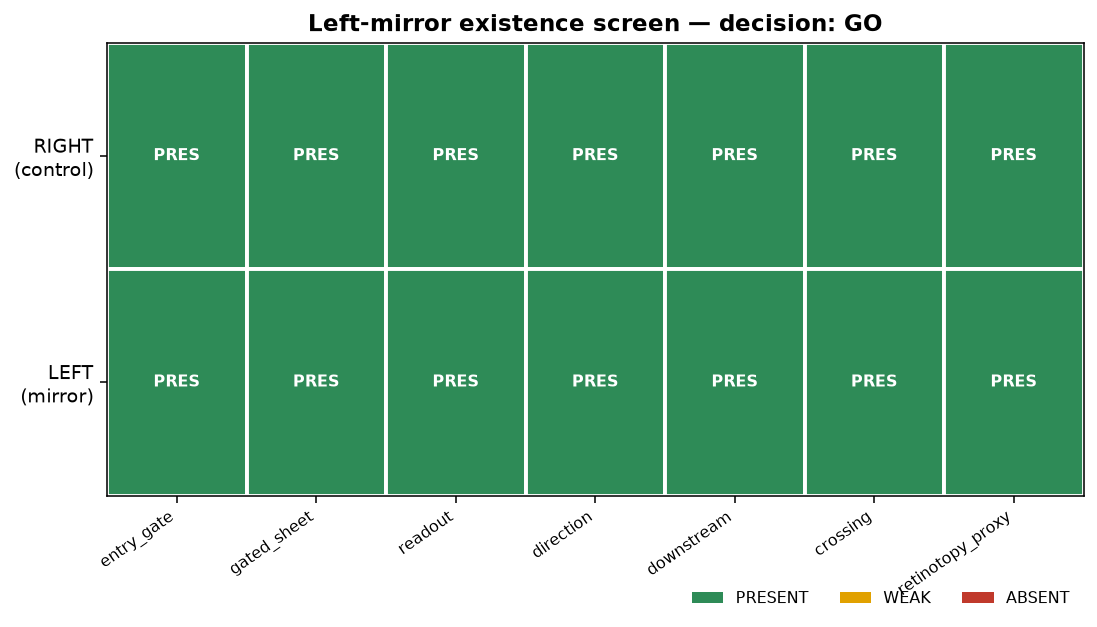
\includegraphics[width=0.9\textwidth]{figures/stage_existence.png}
\caption{Stage-by-stage presence of the figure circuit on each side. Each of the seven stages of
the right circuit (entry gate, gated sheet, readout, direction, downstream reach, contralateral
crossing, and bounded retinotopic pooling) is present on the left as on the right. The decision
to proceed to the full characterisation rested on this measured correspondence.}
\label{fig:stages}
\end{figure}

\begin{figure}[t]
\centering
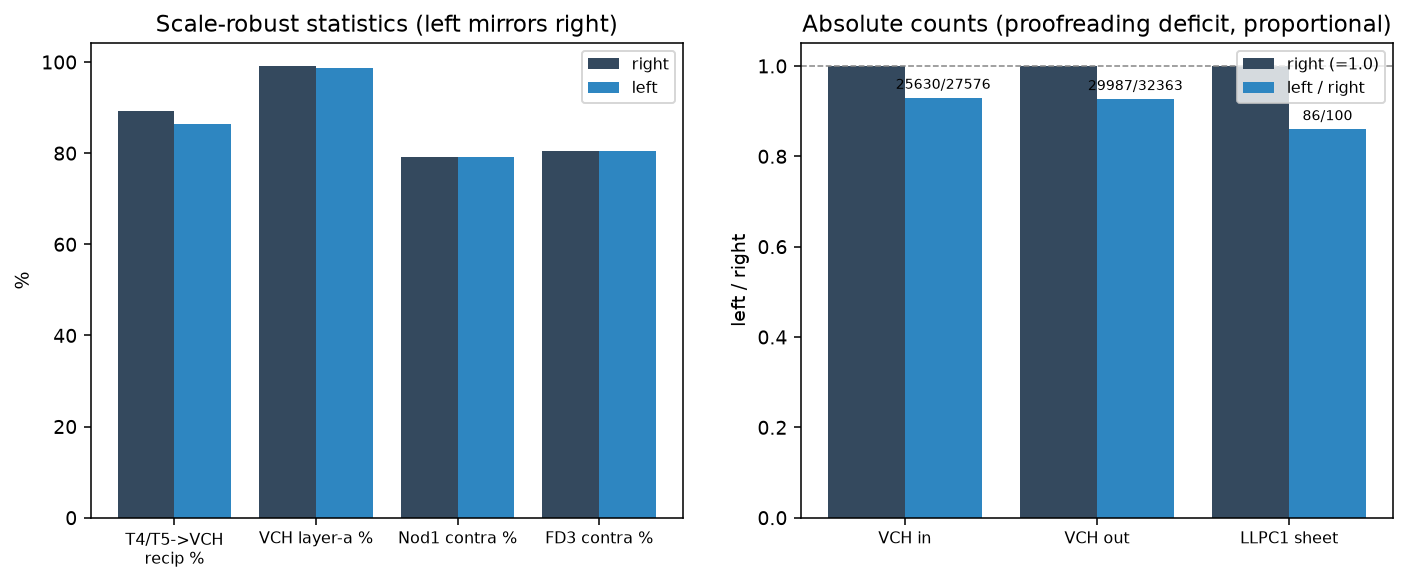
\includegraphics[width=0.95\textwidth]{figures/mirror_comparison.png}
\caption{Left and right values for the count-independent statistics (left panel) and the absolute
counts normalised to the right value (right panel). The fractions, layer compositions, and
contralaterality measures coincide across the hemispheres, while the absolute counts are smaller
on the left by a coherent seven to fourteen percent, consistent with per-hemisphere proofreading
completeness.}
\label{fig:mirror}
\end{figure}

\begin{figure}[t]
\centering
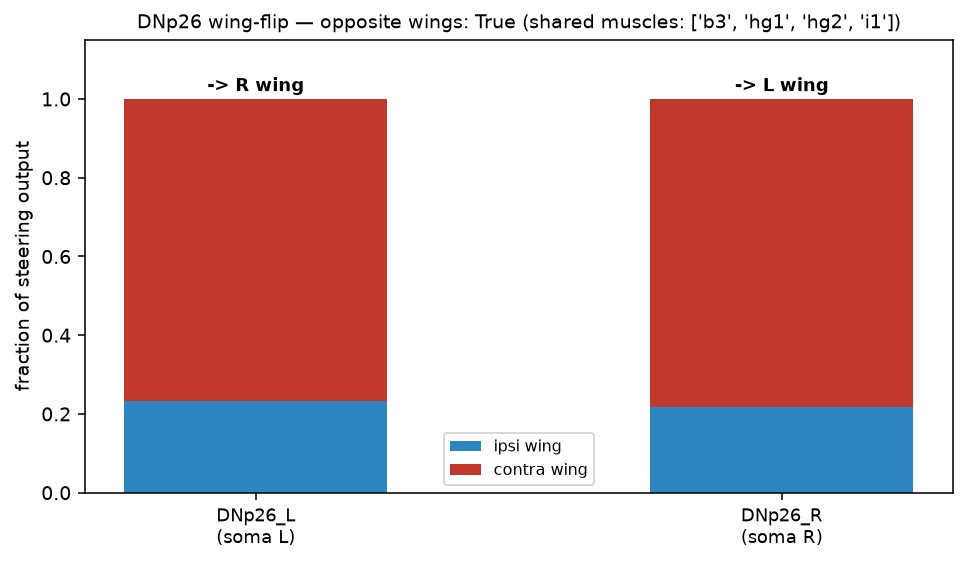
\includegraphics[width=0.8\textwidth]{figures/wing_flip.png}
\caption{The complement. Each DNp26 cell directs the majority of its steering output to the wing
opposite its own soma, through the same hg1, hg2, i1, and b3 muscles. The left-brain figure
circuit addresses the left-soma DNp26 and steers the right wing; the right-brain circuit
addresses the right-soma DNp26 and steers the left wing.}
\label{fig:wing}
\end{figure}

\begin{figure}[t]
\centering
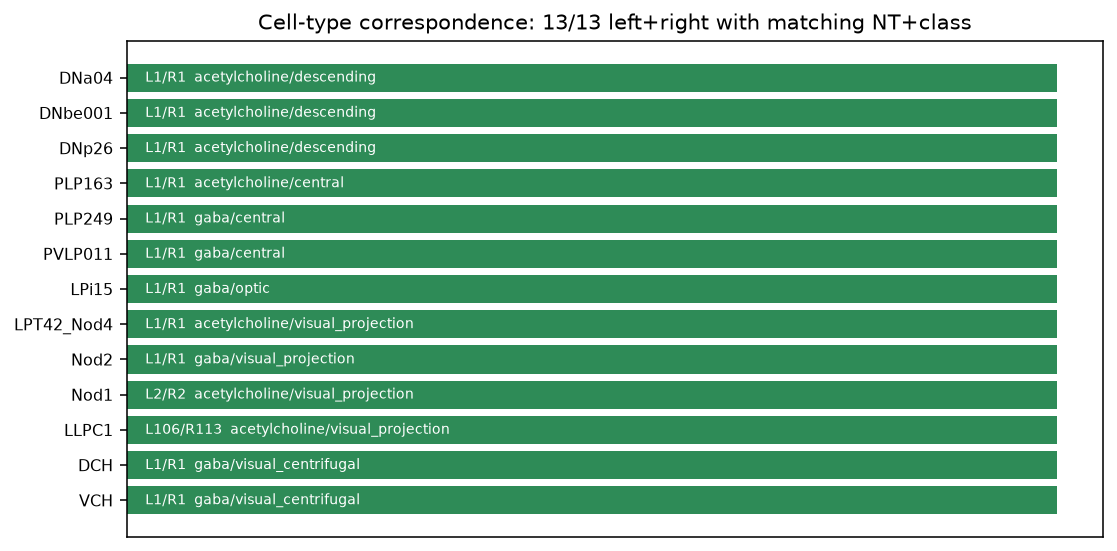
\includegraphics[width=0.9\textwidth]{figures/per_celltype_bars.png}
\caption{Cell-type correspondence. For each named circuit cell type a left and a right cell exist
with matching predicted transmitter and super-class. The correspondence is complete across all
thirteen types.}
\label{fig:celltypes}
\end{figure}

\section*{Data and reproducibility}

All analyses use public connectomic resources. The FlyWire-derived results used materialization
version 783 of \texttt{flywire\_fafb\_public}, with chemical synapses from the
\texttt{synapses\_nt\_v1} table using all synapses and no cleft-score threshold. The motor
read-out used the male whole-CNS connectome (male-cns:v1.0). The two hemispheres were derived
through one parametrised analysis path so that the right-hemisphere derivation reproduces the
companion study exactly and serves as a positive control. The complete per-quantity ledger, the
cell-identity manifest with every root identifier, and the figures are provided alongside this
document in the stage directory. One internal stage, the elimination screen that establishes
LLPC1 as the unique columnar projection sheet driven by the gated field, requires a broadcast
query over roughly five hundred thousand synapses that did not complete within the live query
window; it is independent of the existence and complement results reported here and can be
recomputed when the materialization service is responsive.

\end{document}
